\documentclass[a4j,dvipdfmx]{article}
%Format   -----------------------
\usepackage[utf8]{inputenc}
\usepackage[euler]{textgreek}
\usepackage{enumitem}
\usepackage[margin=30mm]{geometry}
\usepackage{comment}
\usepackage[dvipdfmx]{hyperref}
\usepackage{float}
\usepackage{subcaption}
\usepackage{textcomp}
\usepackage{palatino}
\usepackage{xparse}
%Format   -----------------------

%Circuit ------------------------
%\begin{comment}
\usepackage{amsmath,amssymb}
\usepackage[dvipdfmx]{graphicx}
\usepackage{siunitx}
\usepackage{tikz}
\usepackage{circuitikz}
%\end{comment}
%Circuit ------------------------

%Command ---–--------------------
\renewcommand{\figurename}{図}
%--------------------------------

%Title   ------------------------
\title{実験レポートA1}
\author{東京大学工学部電気電子工学科 03210517\ 藤田 誠之 }
\date{May 15, 2021}
%Title   ------------------------
\renewcommand{\baselinestretch}{1.2}
\begin{document}
\tikzset{component/.style={draw,thick,circle,fill=white,minimum size =0.75cm,inner sep=0pt}}

\maketitle

\section{考察課題}

\begin{enumerate}[label={(\arabic*)}]
  \item 測定レンジと内部抵抗にはどのような関係があるのか、図A1.13を参照しながら推測し、測定結果と比較してみよ。pn接合ダイオードの電流電圧特性が正確に測定されていると思われる領域と、測定系の限界が(補正をしても)測定結果に影響を与えられていると思われる領域を明らかにせよ。
\end{enumerate}
理想的な電圧計と電流計の内部抵抗について考える。


\begin{enumerate}[label={(\arabic*)}]
    \setcounter{enumi}{1}
    \item pn接合ダイオードの電流電圧特性について、測定結果と理論を定量的に比較し、理論からのズレとその要因を考察せよ。
\end{enumerate}

FETトランジスタを以下の回路図のようにつなげ、電圧と電流を測定した。Dは接続していない。このように接続すると、トランジスタはpn接合ダイオードとなる。

\begin{figure}
  \begin{center}
    \begin{circuitikz}[american currents]
     \ctikzset{american inductors}
	  \draw (0,4)
      to[battery1] (0,0)
      to[short] (5,0)
	  to[short] (5,2) 
	  node[component]{V}
	  to[short] (5,4)
	  to[short] (2.5,4) node[component]{A} to [short] (0,4);
	  \draw(5,4)
	  to[short] (6,4);
    \draw(7,2)
	  node[njfet](njfet){}
	  (njfet.base) node[anchor=east] {G}
	  (njfet.collector) node[anchor=south] {D}
	  (njfet.emitter) node[anchor=west] {S};
	  to[short] (3,0);
	  \draw(6,4)
	  to[short] (njfet.base);
    \draw(4,0)
    to[short] (7,0)
    to[short] (njfet.emitter);
	  \draw ($(njfet)-(0.18,0)$) circle [radius=18pt];
    \end{circuitikz}
    \caption{a順方向}
  \end{center}
\end{figure}
ここで、電圧計で計測される電圧は$V_{GS}$、電流計で計測される電流を$I$とし計測されたデータをグラフ化したものが以下である。

\begin{figure}
\begin{center}
\includegraphics[width=12cm]{../graph/figures/data_pn_a_normal.png}
\caption{title)}
\end{center}
\end{figure}

PN接合の特性は一般に以下の式で示される。
$$
I = I_0\left(e^{\frac{qV}{kT}}-1\right)
$$
しかし、実際のPN接合ダイオードでは、結晶欠陥や寄生抵抗などが存在することから、理想的な状態とはかなり異なっている。順バイアス時には、電圧を上げていくに連れ、まず欠陥による再結合により、電流が$e^{\frac{qV}{2kT}}$に比例するようになる。その後、$e^{\frac{qV}{kT}}$に比例した後、高注入効果により再び$e^{\frac{qV}{kT}}$に比例し、最終的には寄生抵抗により電圧と比例関係となるようになる。\\

電流の対数をとったものの図は以下のようになる。
\begin{figure}
  \begin{center}
  \includegraphics[width=12cm]{../graph/figures/data_pn_a_normal_log.png}
  \caption{title)}
  \end{center}
\end{figure}
ここで、青の点の部分はおよそ電流が$e^{\frac{qV}{kT}}$に比例していると考えられる。青い部分の傾きの逆数を最小2乗法で求めると、0.030となった。室温を$\deg{20}$とすると${qV}{kT}=0.026$となるので、誤差率11\%とよく一致していることがわかる。また、赤い部分は電流がおおよそ$e^{\frac{qV}{kT}}$に比例すると考えられるが、この部分の傾きを同じく最小二乗法で計算すると0.13となる。赤の部分に関しては高注入効果及び寄生抵抗により傾きがだんだんと減少していくはずであるので、得られた実験結果は理論と一致しているということができる。

\begin{enumerate}[label={(\arabic*)}]
  \setcounter{enumi}{2}
  \item FETの静特性について理論を調べ、測定値と理論値を定量的に比較した上で、理論からのズレを考察せよ。
\end{enumerate}

pn接合ダイオードの電流電圧特性は、\\
\begin{center}
  三極管領域において
\end{center}
$$
I_D = \mu_nC_{OX}\frac{W}{L}\left((V_{GS}-V_{TH})V_{DS} - \frac{1}{2}V_{DS}^2\right) = \beta\left((V_{GS}-V_{TH})V_{DS} - \frac{1}{2}V_{DS}^2\right)
$$
\begin{center}
    飽和領域において
\end{center}
$$
I_D = \frac{1}{2}\mu_nC_{OX}\frac{W}{L}\left(V_{GS}-V_{TH}\right)^2 = \frac{1}{2}\beta(V_{GS}-V_{TH})^2
$$
\begin{align}
  \mu_n &: \mbox{電子の移動度[m}^2\mbox{/Vs]}\nonumber \\
  C_{OX} &: \mbox{単位面積あたりの酸化膜容量[F/m}^2\mbox{]} \nonumber \\
  W &: \mbox{チャネル幅[m]} \nonumber \\
  L &: \mbox{実効チャネル長[m]} \nonumber \\
  \beta &: \mbox{利得係数} \nonumber
\end{align}
と表すことができる。ここで、今回使用したトランジスタ2SK30ATMのゲート・ドレイン間しゃ断電圧$V_{TH}$($V_{GS(OFF)}$)は規格書によると下限が-0.4V、上限が-5.0Vとなっている。図の回路図のような回路を組み立て、$V_{DS}$を変化させながら$I_D$を測定した結果、得られたデータは図のようになった。

\begin{figure}
  \begin{center}
    \begin{circuitikz}[american currents]
     \ctikzset{american inductors}
    \draw (0,0)
    to[battery1] (0,2)
    to[short] (1,2)
    to[short] (1,1) node[component](v2){V}
    to[short] (1,0)
    to[short] (0,0);
    \draw ($(v2)+(0.4,0)$) node[anchor=west] {$V_{GS}$};
    \draw(4,2.27) node[njfet](njfet){}
    (njfet.base) node[anchor=north] {G}
    (njfet.collector) node[anchor=east] {D}
    (njfet.emitter) node[anchor=east] {S};
    \draw ($(njfet)-(0.18,0)$) circle [radius=18pt];
    \draw (0,2)
    to[short] (njfet.base);
    \draw (1,0)
    to[short] (4,0)
    to[short] (njfet.emitter);
    \draw (njfet.collector)
    to[short] (4,4)
    to[short] (5,4)
    to[short] (5,2)
    node[component](v1){V}
    to[short] (5,0)
    to[short] (4,0);
    \draw ($(v1)+(0.4,0)$) node[anchor=west] {$V_{DS}$};
    \draw (5,4)
    to[short] (6,4)
    node[component]{A}
    to[short] (7,4)
    to[battery1] (7,0)
    to[short] (4,0);
    \end{circuitikz}
    \caption{2}
  \end{center}
\end{figure}

\begin{figure}
  \begin{center}
  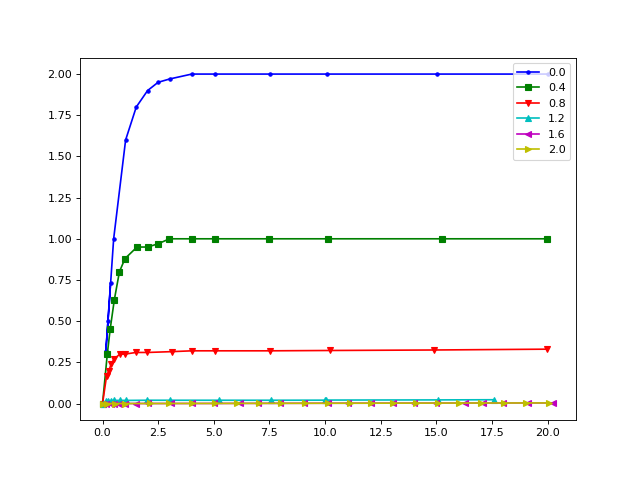
\includegraphics[width=12cm]{../graph/figures/all.png}
  \caption{title}
  \end{center}
\end{figure}

\begin{figure}
  \begin{center}
  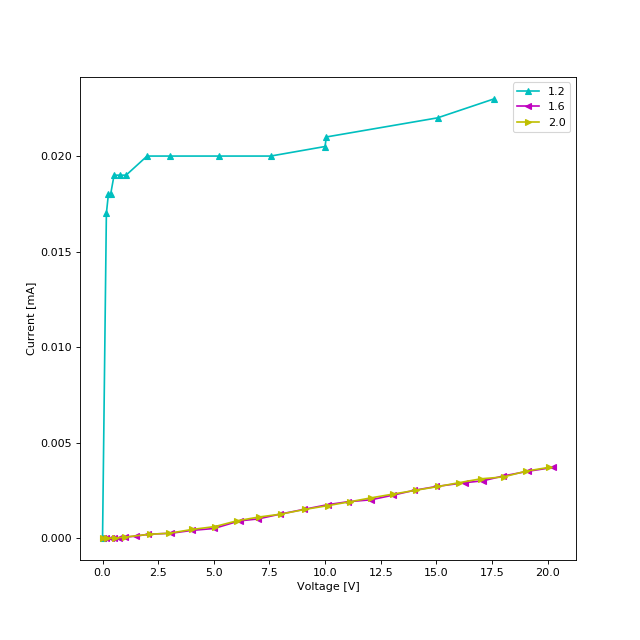
\includegraphics[width=12cm]{../graph/figures/lower.png}
  \caption{title}
  \end{center}
\end{figure}

上記に記した$I_D$の式を用いて、計測結果をフィッティングしようと試みた。$\beta$と$V_{TH}$は理論上$V_{DS}$に関係することのない定数であるとして、まずは飽和領域での値を合わせようとした。\\
フィッティングした結果、$\beta = 2.25, V_{TH} = -1.335$とし、得られた飽和時のドレイン電流は以下の通りである。

\begin{table}[H]
  \begin{center}
    \begin{tabular}{|c|c|c|c|} \hline
      $V_{GS}$[V] & \begin{tabular}{c}$I_D$の飽和時の\\ドレイン電流[mA]\end{tabular}& \begin{tabular}{c}フィッテイング曲線の$I_D$の\\飽和時のドレイン電流[mA]\end{tabular}& 誤差率 \\ \hline
      0.0 & 2.00 & 2.00 & 0.0\% \\ \hline
      -0.4 & 1.00 & 0.984 & 98\% \\ \hline
      -0.8 & 0.33 & 0.322 & 98\% \\ \hline
      -1.2 & 0.023 & 0.021 & 91\% \\ \hline
      \end{tabular}
      \caption{title}
  \end{center}
\end{table}

このように、飽和時のドレイン電流については非常によくフィッティングすることができた。ただ、$V_{TH}=-1.335$としているため、$V_{GS} < -1.335\mbox{V}$となるデータについてはトランジスタがONとなっていないため、上記の式では表せない。これについても、読み取られたデータと合致している。つまり、$V_{GS}$が$V_{TH}$を下回っている$V_{GS} = 1.6, 2.0$については、三極管領域が存在せず、直線でフィッティングできることがわかる。\\
ただし、このフィッティング曲線はピンチオフ電圧の誤差が大きいこともわかる。理論上、ピンチオフ電圧は$V_{p} = V_{GS}-V{TH} = V_{GS} + 1.335$となる。それぞれの$V_{GS}$についての誤差は以下の表の様になる。

\begin{table}[H]
  \begin{center}
    \begin{tabular}{|c|c|c|c|} \hline
      $V_{GS}$[V] & \begin{tabular}{c}データから読み取れた$V_p$\end{tabular} & \begin{tabular}{c}フィッテイング曲線の$V_p$\end{tabular}& 誤差率 \\ \hline
      0.0 & 3.0 & 1.335 & 56\% \\ \hline
      -0.4 & 1.5 & 0.955 & 36\% \\ \hline
      -0.8 & 0.8 & 0.555 & 30\% \\ \hline
      -1.2 & 0.2 & 0.155 & 22\% \\ \hline
      \end{tabular}
      \caption{title}
  \end{center}
\end{table}

このように、とても誤差が大きくなってしまっていることがわかる。ここで、$V_{P} = V_{DS} - V_{TH}$であるから、$V_{TH}$が実際の値よりも大きく測定されたか、$V_{GS}$が実際の値よりも小さく測定されたということが考えられる。$V_{GS}$は直接電圧計を当てて測定しているため、大きな誤差が生じるとは考えにくいため、フィッティングした際に計算された$V_{TH}$の値に大きな誤差があると考えられるが、他のパラメータはよくフィッティングできているため、どうしてこのような結果となったのかをこのレポートの提出までに原因を特定することはできなかった。

\section{参考文献}
『title』\url{<url>} 2021年n月m日アクセス
\end{document}


\begin{comment}
--------------------------------
--見出し
\section{実験方法}
--番号を振る
\begin{enumerate}[label={(\arabic*)}]
\item
--画像の挿入
\begin{figure}[H]
\begin{center}
\includegraphics[width=8cm]{figures/name}
\caption{title)}
\end{center}
\end{figure}

--回路(例)
\begin{figure}[H]
\begin{center}
\begin{circuitikz}[american currents]
\ctikzset{american inductors}
\draw (0,0)
to[sV=V_s$] (0,2)
to[L=L_2$] (6,2)
to[C=$$
to[european resistor=\Omega$] (6,0)
to[short] (3,0);
\end{circuitikz}
\caption{3次規格化0-R型LPF}
\end{center}
\end{figure}

--表
\begin{table}[H]
\begin{center}
\begin{tabular}{|l|l|c||} \hline
11 & 12 & 13 \ \hline
21 & 22 & 23 \ \hline
31 & 32 & 33\ \hline
\end{tabular}
\caption{title}
\end{center}
\end{table}
\end{comment}